\documentclass[11pt]{article}

\usepackage[a4paper,margin=1in]{geometry}
\usepackage{amsmath,amssymb,amsthm}
\usepackage{graphicx}
\usepackage{booktabs}
\usepackage{algorithm}
\usepackage{algpseudocode}
\usepackage[hidelinks]{hyperref}
\usepackage{sudoku}
\usepackage{tikz}

\title{Signed p-adic Residual Encodings of Finite-Domain All-Different Systems\\with a Sudoku Case Study\thanks{This article presents material that also appears as a chapter of the author's PhD dissertation (Australian National University, in preparation); it is the standalone version of that work.}}
\author{Greg Baker\\\small School of Computing, Australian National University\\\small Canberra, Australia\\\small \href{mailto:greg.baker@anu.edu.au}{greg.baker@anu.edu.au}\\\small ORCID: \href{https://orcid.org/0000-0002-6910-3011}{0000-0002-6910-3011}}
\date{}
\hypersetup{
    pdftitle={Signed p-adic Residual Encodings of Finite-Domain All-Different Systems with a Sudoku Case Study},
    pdfauthor={Greg Baker},
    pdfkeywords={p-adic regression, signed residual objectives, all-different constraints, list colouring, Sudoku}
}

\newtheorem{theorem}{Theorem}
\newtheorem{corollary}[theorem]{Corollary}
\newtheorem{lemma}{Lemma}
\newtheorem{definition}{Definition}
\newcommand{\sudokublank}{\phantom{0}}
\newcommand{\papersudokustyle}{%
    \setlength{\sudokusize}{6.2cm}%
    \setlength{\sudokuthinline}{0.8pt}%
    \setlength{\sudokuthickline}{2.8pt}%
    \renewcommand*\sudokuformat[1]{\Large\sffamily ##1}%
}

\begin{document}
\maketitle

\begin{abstract}
We encode finite-domain all-different systems as signed synthetic \(p\)-adic residual objectives, with Sudoku as a worked example. Given a graph whose vertices carry finite allowed sets and whose edges require unequal assignments, positive synthetic observations create unary domain wells and negative synthetic observations reward pairwise inequality. For primes \(p>q\), every nonzero difference between values in \(\{1,\dots,q\}\) has \(p\)-adic norm \(1\). On domain-respecting states, the objective is therefore an additive constant plus the edge-conflict count. Its global minimisers are exactly the domain-respecting assignments that maximise the number of unequal edges. When the associated list-colouring instance is satisfiable, these minimisers are precisely its proper list-colourings.

Standard Sudoku is a direct instance: there is one variable per cell, singleton domains on clue cells, and edges between cells that share a row, column, or box. The construction uses the original \(81\) cell variables rather than a one-hot lift to \(729\) Boolean indicators. The Sudoku section is not a solver proposal; it spells out the encoding in a case where the variables, domains, and all-different constraints are familiar. The word ``regression'' refers to the affine residual form of the objective, not to an ordinary positive-weight statistical loss.
\end{abstract}

\noindent\textbf{Keywords:} p-adic regression; signed residual objectives; all-different constraints; list colouring; Sudoku

\section{Introduction and prior work}


This paper encodes finite-domain all-different systems as signed synthetic \(p\)-adic residual objectives, with Sudoku as a worked example. The representation keeps one variable per semantic object, uses the same finite domain as the original problem, and enforces both domain membership and pairwise distinctness in one objective.

All signed objectives in this paper are optimised over \(\mathbb Z_p^n\). On this domain every affine residual is bounded by \(1\). Once \(p>q\), the same residual also becomes an exact \(0/1\) equality indicator on the intended finite alphabet. The restriction to \(\mathbb Z_p^n\) is mainly a modelling choice, not a way to hide an unbounded objective: although a single negative term \(-|x_i-x_j|_p\) is unbounded below over \(\mathbb Q_p^n\), the objectives constructed here remain bounded below on \(\mathbb Q_p^n\). The same domination condition that forces digit-snapping, \(\lambda>\Delta\), also dominates the total inequality reward.

Two earlier results motivate the construction:
\begin{itemize}
    \item A structural result on $p$-adic linear regression \cite{baker2025padic}: an optimal hyperplane is supported by $n+1$ data points.
    \item A complexity result on $p$-adic linear regression \cite{baker2026nphard}: the problem is NP-hard, via an embedding of \textsc{Max-Cut} using positive pinning points that snap coefficients to $\{0,1\}$.
\end{itemize}
Recent work in \emph{p-Adic Numbers, Ultrametric Analysis and Applications} connects \(p\)-adic methods with regression structure and optimisation \cite{baker2025padic,zubarev2025padic}. Mihara studies a different regression regime: polynomial regression with digitwise noise \cite{mihara2026polyreg}, and a probabilistic linear-regression algorithm that estimates the digits of one hidden affine law from random samples with sparse digitwise corruption \cite{mihara2026digitwise}.

Mihara also generalises Baker's forcing method from \(p=2\) to arbitrary fixed primes \cite{mihara2026forcing}. For a product domain \(C=\prod_i B_i\) with \(B_i\subseteq\{0,\ldots,p-1\}\), his forcing theorem adds positive unary wells and identifies global optima with those of a nonnegative discrete objective on \(C\), subject to a concentration hypothesis; he consequently proves ordinary \(p\)-adic linear regression NP-hard for every fixed prime. Thus arbitrary finite-alphabet positive pinning is not the distinction of the present construction. The new ingredient here is the signed affine interaction layer: a coordinatewise domination condition permits negative inequality rewards, and the resulting global minimisers are exactly the minimum-conflict list-colourings or all-different assignments on the native finite-domain variables. Section~\ref{sec:mihara-digitwise} explains why Mihara's digitwise-noise linear-regression algorithm is adjacent but not a solver for the Sudoku or Boolean-CSP objectives studied here.

Negative signed residual terms do not have the usual interpretation of Euclidean least-squares terms. Classical generalized ridge regression allowed negative ridge parameters \cite{hua1983negative}; later work found zero or negative risk-optimal ridge parameters in overparameterised models \cite{kobak2020negative} and under distribution shift \cite{patil2024oodridge}. Related anti-shrinkage effects appear in Gaussian model-uncertainty formulations \cite{wiesel2008gaussian} and in multivariate climate downscaling \cite{cannon2009negative}. These results do not justify the present construction by analogy. They only show that negative quadratic penalties are not, by themselves, incoherent. In the \(p\)-adic construction below, the reason they are usable is sharper: on \(\mathbb Z_p^n\), the residuals are bounded, and on the intended finite domain they become equality indicators.

From the constraint-programming side, the construction is close to weighted CSP / Max-CSP penalty functions, graph-colouring energy models, and Ising/Potts/QUBO encodings of discrete optimisation. Sudoku itself is routinely formulated using exact cover, SAT, or \emph{alldifferent} constraints \cite{knuth2000dancing,simonis2005sudoku,lynce2006sudoku}. The feature specific to this paper is the affine \(p\)-adic residual form. Once \(p\) is larger than the finite domain and the unary wells snap the variables to their allowed values, each residual \(|x_i-x_j|_p\) is an equality/inequality indicator on the original domain. The same mechanism also handles clauses: after Boolean pinning, a \(3\)-CNF clause is one forbidden affine equality, so a signed residual can reward its satisfaction.

\section{Preliminaries}

\subsection{p-adic integers and norms}
Fix a prime $p$. The $p$-adic valuation $v_p(n)$ of an integer $n\neq 0$ is the exponent of $p$ in its factorisation, and the $p$-adic absolute value is
\[
|n|_p = p^{-v_p(n)}, \qquad |0|_p = 0.
\]
We will work in the $p$-adic integers $\mathbb{Z}_p$, where all norms satisfy $|x|_p\le 1$. The key choice for Sudoku is to take $p>9$ (e.g.\ $p=11$), so that the $p$-adic absolute value of any Sudoku digit or digit difference is always \(0\) or \(1\).

For comparison, note that the discrete metric \(d_{\mathrm{disc}}(s,t):=\mathbf 1_{s\neq t}\) is also an ultrametric. We return to a companion discrete-metric version of the reduction after the main correctness theorem.



\subsection{List colouring}
Many finite-domain constraint systems built from all-different conditions can be viewed as list-colouring problems on a graph. Each variable $x_i$ is assigned a value from a finite allowed set $D_i$, and an edge $\{i,j\}$ expresses the preference or requirement that $x_i\neq x_j$. Thus an all-different constraint of arity \(r\) contributes the \(\binom{r}{2}\) pairwise edges of its primal-graph clique; this paper uses that pairwise primal graph, not global \emph{alldifferent} propagation.

Figure~\ref{fig:list-colouring-example} gives a concrete toy instance.

\begin{figure}[b]
\centering
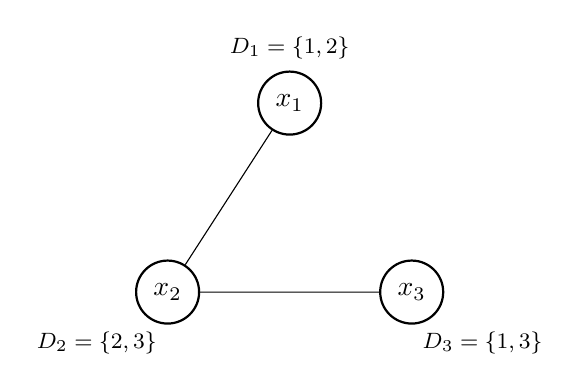
\begin{tikzpicture}[vertex/.style={circle,draw,thick,minimum size=8mm,inner sep=0pt}]
\node[vertex] (x1) at (0,1.45) {$x_1$};
\node[vertex] (x2) at (-1.55,-0.95) {$x_2$};
\node[vertex] (x3) at (1.55,-0.95) {$x_3$};
\draw (x1) -- (x2) -- (x3);
\node[font=\footnotesize] at (0,2.15) {$D_1=\{1,2\}$};
\node[font=\footnotesize] at (-2.45,-1.6) {$D_2=\{2,3\}$};
\node[font=\footnotesize] at (2.45,-1.6) {$D_3=\{1,3\}$};
\end{tikzpicture}
\caption{A tiny list-colouring instance. The assignment \(x_1=1\), \(x_2=2\), \(x_3=3\) respects the domains and makes every edge unequal.}
\label{fig:list-colouring-example}
\end{figure}

One solution is \(x=(1,2,3)\).

\subsection{Residual-objective formulation}

The equivalent dataset for the toy instance in Figure~\ref{fig:list-colouring-example} is shown in Figure~\ref{fig:list-colouring-regression}.

Its synthetic dataset has six positive observations, one for each allowed value in the three domains, and two negative observations, one for each edge. At the coefficient vector \(x=(1,2,3)\), every edge reward is active and the unary term attains its baseline value. 

\begin{figure}[t]
\centering
\small
\begin{tabular}{@{}llp{0.3\linewidth}@{}}
\toprule
Type & Synthetic observations & Role \\
\midrule
positive & $(+1,e_1,1,3)$ & pin $x_1$ to $D_1$ \\
positive & $(+1,e_1,2,3)$ & pin $x_1$ to $D_1$ \\
positive & $(+1,e_2,2,3)$ & pin $x_2$ to $D_2$ \\
positive & $(+1,e_2,3,3)$ & pin $x_2$ to $D_2$ \\
positive & $(+1,e_3,1,3)$ & pin $x_3$ to $D_3$ \\
positive & $(+1,e_3,3,3)$ & pin $x_3$ to $D_3$ \\
negative & $(-1,e_1-e_2,0,1)$ & reward $x_1\neq x_2$ \\
negative & $(-1,e_2-e_3,0,1)$ & reward $x_2\neq x_3$ \\
\bottomrule
\end{tabular}
\caption{Synthetic dataset for the toy list-colouring instance in Figure~\ref{fig:list-colouring-example}. Here \(e_1,e_2,e_3\) denote the standard basis vectors of \(\mathbb Z^3\).}
\label{fig:list-colouring-regression}
\end{figure}

\section{A general all-different residual-objective template}
\label{construction}

Over $\mathbb{Z}_p$ with $p>q$, once values are restricted to $\{1,\dots,q\}$, every nonzero difference has norm $1$.

\begin{definition}[Signed synthetic $p$-adic residual dataset]
\label{def:signed-dataset}
For parameters \(x\in \mathbb Z_p^n\), a signed weighted affine observation is a quadruple \((\sigma,u,b,\gamma)\), where \(\sigma\in\{+1,-1\}\) is the sign, \(u\in\mathbb Z^n\) is the feature vector, \(b\in\mathbb Z\) is the target, and \(\gamma>0\) is the weight. It contributes the term
\[
\sigma\gamma\,|u^\top x-b|_p
\]
to the loss; formally, this is the $p$-adic analogue of a weighted Euclidean residual term.
\end{definition}

Throughout this paper \(x\) ranges over \(\mathbb Z_p^n\). Since \(u\in\mathbb Z^n\), \(b\in\mathbb Z\), and \(x\in\mathbb Z_p^n\), each residual \(u^\top x-b\) lies in \(\mathbb Z_p\), and hence \(|u^\top x-b|_p\le 1\). Every finite signed objective considered here is therefore bounded on its stated domain.

We will use the phrase \emph{signed $p$-adic residual objective} for sums of such terms. The word ``regression'' refers to the affine residual form of the objective; because negative weights are allowed, the resulting functional is an optimisation objective rather than a statistical loss in the usual positive-weight sense.

\begin{definition}[Positive/negative observations]
A signed weighted affine observation \((\sigma,u,b,\gamma)\) is \emph{positive} if \(\sigma=+1\) and \emph{negative} if \(\sigma=-1\). In the constructions below, positive observations serve as pinning terms and negative observations serve as reward terms.
\end{definition}

\begin{theorem}[Finite-domain signed affine compiler template]
\label{thm:compiler-template}
Fix a prime \(p\). Let \(D_i\subseteq\mathbb Z\) be finite nonempty sets whose elements are pairwise incongruent modulo \(p\), and put
\[
D:=\prod_{i=1}^n D_i\subseteq\mathbb Z_p^n.
\]
For each coordinate \(i\), choose a pinning weight \(\lambda_i>0\). Let \(\mathcal T\) be a finite family of signed affine observations
\[
(\sigma_\ell,u_\ell,b_\ell,\gamma_\ell),
\qquad
\sigma_\ell\in\{\pm1\},\quad u_\ell\in\mathbb Z^n,\quad b_\ell\in\mathbb Z,\quad \gamma_\ell>0,
\]
and define
\[
L(x):=
\sum_{i=1}^n\lambda_i\sum_{a\in D_i}|x_i-a|_p
\;+\;
\sum_{\ell\in\mathcal T}\sigma_\ell\gamma_\ell |u_\ell^\top x-b_\ell|_p.
\]
Assume that, for every coordinate \(i\),
\[
\lambda_i>\sum_{\ell:\,(u_\ell)_i\neq 0}\gamma_\ell,
\]
and that, for every \(x\in D\) and every \(\ell\in\mathcal T\), the residual \(u_\ell^\top x-b_\ell\) is either \(0\) or a \(p\)-adic unit. Then \(L\) attains its global minimum on \(D\), and every global minimiser lies in \(D\). On \(D\), \(L\) is a constant plus a finite signed objective whose interaction terms have values \(0\) and \(\sigma_\ell\gamma_\ell\).
\end{theorem}

\begin{proof}
Suppose \(x_i\notin D_i\). If \(x_i\) is congruent modulo \(p\) to an element of \(D_i\), let \(b\) be that element; otherwise choose any \(b\in D_i\). Let \(x'\) be obtained from \(x\) by replacing \(x_i\) with \(b\).

The \(i\)-th unary sum decreases by at least \(\lambda_i|x_i-b|_p\). Indeed, if \(x_i\equiv b\pmod p\), then the only changed unary contribution below \(1\) is \(|x_i-b|_p\). If \(x_i\) is congruent to no element of \(D_i\), then \(|x_i-a|_p=1\) for all \(a\in D_i\), while the unary sum at \(b\) has one zero term and all other terms equal to \(1\); in this case \(|x_i-b|_p=1\).

For an interaction term with \((u_\ell)_i\neq0\), write \(r_\ell'=u_\ell^\top x'-b_\ell\). Then
\[
u_\ell^\top x-b_\ell=r_\ell'+(u_\ell)_i(x_i-b).
\]
Since \((u_\ell)_i\in\mathbb Z\), \(|(u_\ell)_i|_p\le1\), and the ultrametric inequality gives
\[
\bigl||u_\ell^\top x-b_\ell|_p-|r_\ell'|_p\bigr|
\le |x_i-b|_p.
\]
Thus the total interaction increase caused by changing coordinate \(i\) is at most
\[
\sum_{\ell:\,(u_\ell)_i\neq0}\gamma_\ell |x_i-b|_p.
\]
By the assumed domination inequality, \(L(x')<L(x)\). Repeating this coordinate-snapping step gives a point of \(D\) with smaller loss than any starting point outside \(D\). Since \(D\) is finite, the global minimum is attained on \(D\), and no global minimiser lies outside \(D\).

On \(D\), every unary sum is constant: exactly one term is zero and the rest are units. The second assumption says each interaction residual is either zero or a unit, so each signed interaction term is either \(0\) or \(\sigma_\ell\gamma_\ell\). This proves the stated finite-domain form of \(L|_D\).
\end{proof}

\begin{definition}[Synthetic dataset for list-colouring]
\label{def:list-dataset}
Let \(V=\{1,\dots,n\}\), let \(G=(V,E)\) be a finite graph, let \(D_i\subseteq \{1,\dots,q\}\) be nonempty allowed sets, and fix a prime \(p>q\). Define
\[
w_{ii}:=0,
\qquad
w_{ij}:=
\begin{cases}
1, & \{i,j\}\in E,\\
0, & \{i,j\}\notin E,
\end{cases}
\qquad (i\neq j),
\]
let \(\Delta:=\max_{i\in V}\sum_{j=1}^n w_{ij}\), and set \(\lambda:=1+\Delta\). Writing \(e_1,\dots,e_n\) for the standard basis vectors of \(\mathbb Z^n\), define
\[
\mathcal S^+ := \{(+1,e_i,a,\lambda): i\in V,\ a\in D_i\},
\]
\[
\mathcal S^- := \{(-1,e_i-e_j,0,1): 1\le i<j\le n,\ w_{ij}=1\}.
\]
Set \(\mathcal S:=\mathcal S^+\sqcup\mathcal S^-\).
\end{definition}

The theorem is stated for a simple graph, so \(w_{ij}\in\{0,1\}\). An edge-weighted version is obtained by replacing the unit negative observation on edge \(\{i,j\}\) with weight \(c_{ij}>0\) and choosing the pinning weight larger than \(\max_i\sum_j c_{ij}\), but the binary case is the one needed here.

\begin{definition}[Loss associated with the list-colouring dataset]
\label{def:list-loss}
For \(\mathcal S\) as in Definition~\ref{def:list-dataset}, define
\[
L_{\mathcal S}(x)
=
\lambda\sum_{i=1}^n \sum_{a\in D_i}|x_i-a|_p
-\sum_{1\le i<j\le n} w_{ij}|x_i-x_j|_p.
\]
\end{definition}

This dataset has exactly \(\sum_{i=1}^n |D_i|\) positive observations and \(|E|\) negative observations, so it is computable in time \(O(\sum_i |D_i|+|E|)\). The positive observations pin coordinates to allowed values, and the negative observations reward inequality across edges.

Each positive observation \((+1,e_i,a,\lambda)\) contributes \(\lambda|x_i-a|_p\) to the loss, and each negative observation \((-1,e_i-e_j,0,1)\) contributes \(-|x_i-x_j|_p\) to the loss. Summing them yields the displayed loss. The size bound and runtime are immediate from the explicit definitions.

The compiler template already implies that minimisers snap to the finite alphabet, because the pinning weight is larger than the degree of every vertex. The next proof records the stronger fact needed for all-different systems: after snapping, the objective is exactly a constant plus the edge-conflict count.

\subsection{Correctness}
Since \(p>q\), the residues of \(1,\dots,q\) are distinct modulo \(p\). In particular, for any fixed \(i\in V\) and any \(t\in\mathbb Z_p\), there is at most one \(a\in D_i\) with \(t\equiv a\pmod p\).

First we record the simple observation that, on \(\{1,\dots,q\}\), the \(p\)-adic norm detects inequality exactly.

\begin{lemma}[Edge terms become inequality indicators on the domain]
\label{lem:edge-indicator}
If \(x_i,x_j\in \{1,\dots,q\}\) and \(p>q\), then
\[
|x_i-x_j|_p=
\begin{cases}
0,&x_i=x_j,\\
1,&x_i\neq x_j.
\end{cases}
\]
\end{lemma}

\begin{proof}
If \(x_i=x_j\) then the difference is zero. If \(x_i\neq x_j\), then \(1\le |x_i-x_j|\le q-1<p\), so \(p\nmid (x_i-x_j)\) and therefore \(|x_i-x_j|_p=1\).
\end{proof}

We next prove a digit-snapping lemma: if \(x\) minimises \(L_{\mathcal S}\), then each coordinate \(x_i\) lies in \(D_i\). The explicit unary-well formula makes that argument transparent.

\begin{lemma}[Unary wells]
\label{lem:unary-well}
For \(i\in V\), define
\[
U_i(t):=\sum_{a\in D_i}|t-a|_p
\qquad (t\in\mathbb Z_p).
\]
Then \(U_i(t)\ge |D_i|-1\), with equality if and only if \(t\in D_i\).
\end{lemma}

\begin{proof}
If \(t\in D_i\), then one summand in \(U_i(t)\) is \(0\), and the remaining \(|D_i|-1\) summands are \(1\), so \(U_i(t)=|D_i|-1\).

If \(t\notin D_i\) but \(t\equiv b \pmod p\) for some \(b\in D_i\), then \(0<|t-b|_p<1\), while for every \(a\in D_i\setminus\{b\}\) we have \(t-a\equiv b-a\not\equiv 0\pmod p\), so \(|t-a|_p=1\). Hence
\[
U_i(t)=(|D_i|-1)+|t-b|_p > |D_i|-1.
\]

If \(t\) is congruent modulo \(p\) to no element of \(D_i\), then \(|t-a|_p=1\) for all \(a\in D_i\), so \(U_i(t)=|D_i|>|D_i|-1\).
\end{proof}

\begin{lemma}[Digit-snapping lemma]
\label{lem:digit-snapping}
Let \(x\in\mathbb Z_p^n\). Suppose there exists \(i\in V\) with \(x_i\notin D_i\). Choose \(b\in D_i\) as follows: if \(x_i\) is congruent modulo \(p\) to an element of \(D_i\), take that unique element; otherwise choose any \(b\in D_i\). Let \(x'\) be obtained from \(x\) by replacing \(x_i\) with \(b\). Then
\[
L_{\mathcal S}(x')<L_{\mathcal S}(x).
\]
\end{lemma}

\begin{proof}
The positive part of the loss changes by
\[
\lambda\left(\sum_{a\in D_i}|b-a|_p-\sum_{a\in D_i}|x_i-a|_p\right).
\]
There are two cases to consider.

If \(x_i\) is congruent modulo \(p\) to no element of \(D_i\), then \(|x_i-a|_p=1\) for every \(a\in D_i\), so \(\sum_{a\in D_i}|x_i-a|_p=|D_i|\). On the other hand, one summand in \(\sum_{a\in D_i}|b-a|_p\) is \(0\) and the remaining \(|D_i|-1\) summands are \(1\), so \(\sum_{a\in D_i}|b-a|_p=|D_i|-1\). Hence the positive change is \(-\lambda\). Since \(|x_i-b|_p=1\) in this case, this is at most \(-\lambda |x_i-b|_p\).

If \(x_i\equiv b \pmod p\) for some \(b\in D_i\), then \(\sum_{a\in D_i}|b-a|_p=|D_i|-1\), whereas
\[
\sum_{a\in D_i}|x_i-a|_p=(|D_i|-1)+|x_i-b|_p.
\]
Hence the positive change is \(-\lambda |x_i-b|_p\).

For each \(j\in V\), the corresponding negative component changes by
\[
w_{ij}\bigl(|x_i-x_j|_p-|b-x_j|_p\bigr).
\]
By the ultrametric inequality,
\[
|x_i-x_j|_p \le \max\bigl(|x_i-b|_p,\ |b-x_j|_p\bigr),
\]
so
\[
|x_i-x_j|_p-|b-x_j|_p \le |x_i-b|_p.
\]
Summing over all \(j\in V\),
\[
L_{\mathcal S}(x')-L_{\mathcal S}(x)
\le
\left(-\lambda+\sum_{j=1}^n w_{ij}\right)|x_i-b|_p
\le
-|x_i-b|_p
<
0.
\]
\end{proof}

On domain-respecting assignments, the loss is an additive constant plus the conflict count.

\begin{theorem}[Correctness of the synthetic reduction]
\label{thm:all-different}
For the dataset \(\mathcal S=\mathcal S^+\sqcup\mathcal S^-\) from Definition~\ref{def:list-dataset} and the loss from Definition~\ref{def:list-loss}, every global minimiser of \(L_{\mathcal S}\) lies in \(\prod_{i=1}^n D_i\). On \(\prod_{i=1}^n D_i\),
\[
L_{\mathcal S}(x)
=
\lambda\sum_{i=1}^n (|D_i|-1)
-|E|
+\sum_{1\le i<j\le n} w_{ij}\mathbf 1_{x_i=x_j}.
\]
Consequently, the global minimisers are exactly the domain-respecting assignments that minimise the conflict sum \(\sum_{1\le i<j\le n} w_{ij}\mathbf 1_{x_i=x_j}\), or equivalently maximise the number of unequal edges. In particular, if the list-colouring instance \((G,(D_i)_{i=1}^n)\) is satisfiable, then this minimum conflict sum is \(0\), and the global minimisers are exactly its proper list-colourings.
\end{theorem}

\begin{proof}
By Lemma~\ref{lem:digit-snapping}, any point with some coordinate outside its domain can be improved by snapping that coordinate into the domain. Therefore every global minimiser lies in \(\prod_i D_i\). If \(x\in \prod_i D_i\), then Lemma~\ref{lem:unary-well} gives \(U_i(x_i)=|D_i|-1\) for every \(i\), and Lemma~\ref{lem:edge-indicator} gives
\[
|x_i-x_j|_p=\mathbf 1_{x_i\neq x_j}
\qquad (1\le i<j\le n).
\]
Since \(\mathbf 1_{x_i\neq x_j}=1-\mathbf 1_{x_i=x_j}\) on every edge, substituting these identities into \(L_{\mathcal S}\) yields the displayed formula. A global minimiser exists: \(L_{\mathcal S}\) takes only finitely many values on the finite set \(\prod_i D_i\), and by the previous paragraph no point outside \(\prod_i D_i\) can be a global minimiser, so the global minimum is attained on \(\prod_i D_i\). There the displayed formula is an additive constant plus the conflict sum, so a domain-respecting assignment is a global minimiser if and only if it attains the least possible conflict sum; this is the stated ``exactly'' characterisation in both directions. In particular, if \((G,(D_i)_{i=1}^n)\) is satisfiable the least conflict sum is \(0\), and the global minimisers are exactly its proper list-colourings.
\end{proof}

\begin{corollary}
\label{cor:all-different-csp}
Any finite-domain all-different constraint system can be encoded, in polynomial time, as a signed weighted synthetic $p$-adic residual objective whose global minimisers are exactly the domain-respecting assignments with minimum conflict count. If the constraint system is satisfiable, these minimisers are exactly its satisfying assignments.
\end{corollary}

\begin{proof}
Given an all-different constraint system, form its primal graph: the vertices are the variables, and two variables are adjacent if they appear together in some all-different constraint. The satisfying assignments are exactly the proper list-colourings of this graph, with the variable domains as lists, and the minimum-conflict assignments are exactly the domain-respecting assignments minimising the corresponding edge-conflict sum. Apply Definitions~\ref{def:list-dataset} and \ref{def:list-loss}, and Theorem~\ref{thm:all-different}.
\end{proof}

\paragraph{Unsatisfiable instances and minimum conflicts.}
The characterisation holds even when the instance has no proper list-colouring: there the global minimisers are the domain-respecting assignments of least conflict count. For example, take the triangle \(K_3\) with all three lists equal to \(\{1,2\}\). No proper \(2\)-colouring of \(K_3\) exists, so every domain-respecting assignment leaves at least one edge monochromatic. Here \(\Delta=2\), so \(\lambda=3\), and by Theorem~\ref{thm:all-different} the global minimisers are exactly the assignments with a single conflict, at loss \(\lambda\sum_i(|D_i|-1)-|E|+1=3\cdot 3-3+1=7\). This Max-CSP regime is distinct from the satisfiable case, and it is exercised directly by the interactive browser demonstration described in the code-and-data statement below: a search that settles above the floor is displaying a minimum-conflict state.

\paragraph{Relation to Potts energies.}
On domain-respecting states the objective equals, up to the additive constant \(\lambda\sum_i(|D_i|-1)-|E|\), the number of monochromatic edges \(\sum_{\{i,j\}\in E}\mathbf 1_{x_i=x_j}\), which is the energy of an antiferromagnetic \(q\)-state Potts model on \(G\) with the lists \(D_i\) as local state constraints. The construction does not alter that energy landscape; its content is the representation of this Potts/Max-CSP energy as a signed affine \(p\)-adic residual objective on the native finite-domain variables.

\paragraph{Discrete-metric variant.}
The same synthetic dataset also works with the discrete metric
\[
d_{\mathrm{disc}}(s,t):=\mathbf 1_{s\neq t}.
\]
If each residual \(|u^\top x-b|_p\) is replaced by \(d_{\mathrm{disc}}(u^\top x,b)\), then the loss becomes
\[
L_{\mathcal S}^{\mathrm{disc}}(x)
=
\lambda\sum_{i=1}^n\sum_{a\in D_i}\mathbf 1_{x_i\neq a}
\;-\;
\sum_{1\le i<j\le n} w_{ij}\mathbf 1_{x_i\neq x_j}.
\]
The unary wells satisfy
\[
U_i^{\mathrm{disc}}(t):=\sum_{a\in D_i}\mathbf 1_{t\neq a}
=
\begin{cases}
|D_i|-1, & t\in D_i,\\
|D_i|, & t\notin D_i.
\end{cases}
\]
Hence replacing any \(x_i\notin D_i\) by a value \(b\in D_i\) decreases the positive part by exactly \(\lambda\), while the total increase in the negative part is at most \(\sum_j w_{ij}\le \Delta\). Since \(\lambda=1+\Delta\), the same snapping argument goes through. Therefore the conclusions of Theorem~\ref{thm:all-different} and Corollary~\ref{cor:all-different-csp} remain valid for the discrete metric as well. The \(p\)-adic case remains the main one because it realises the same indicator behaviour inside the affine \(p\)-adic regression framework used throughout the paper.

\paragraph{Boolean clause rewards.}
The same signed-residual idea also applies beyond all-different constraints. Let
\[
\Phi=\bigwedge_{r=1}^{m} C_r
\]
be a \(3\)-CNF formula on variables \(z_1,\dots,z_n\), and encode truth values by
\[
x_i=0 \iff z_i \text{ is true},
\qquad
x_i=1 \iff z_i \text{ is false}.
\]
For a literal \(\lambda\) on variable \(z_i\), define its failure indicator by
\[
\delta(\lambda;x)=
\begin{cases}
x_i, & \lambda=z_i,\\
1-x_i, & \lambda=\neg z_i.
\end{cases}
\]
Then for a clause \(C=(\lambda_1\vee \lambda_2\vee \lambda_3)\),
\[
C(x)\text{ is false}
\iff
\delta(\lambda_1;x)+\delta(\lambda_2;x)+\delta(\lambda_3;x)=3.
\]
After moving constants to the right-hand side, this means that there are \(u_C\in\mathbb Z^n\) and \(t_C\in\mathbb Z\) such that
\[
C(x)\text{ is true}
\iff
u_C^\top x\neq t_C.
\]
Here \(u_C\) records the \(\pm 1\) literal coefficients, and \(t_C=3-k\), where \(k\) is the number of negated literals in the clause. The translation is mechanical: a positive literal contributes \(+x_i\), a negated literal contributes \(-x_i\), and the forbidden right-hand side is \(3-k\). For example,
\[
(z_1\vee z_2\vee \neg z_3)
\leadsto
x_1+x_2-x_3\neq 2.
\]
If \(p>3\) and \(x\in\{0,1\}^n\), then \(u_C^\top x-t_C\) is \(0\) when \(C\) is false and one of \(-1,-2,-3\) when \(C\) is true, so
\[
|u_C^\top x-t_C|_p=\mathbf 1_{C(x)\text{ is true}}.
\]
Thus a negative observation \((-1,u_C,t_C,1)\) rewards satisfaction of the clause. If \(\Delta\) is the maximum number of clauses containing any variable and \(\alpha>\Delta\), then
\[
L_\Phi(x)
=
\alpha\sum_{i=1}^{n}\bigl(|x_i|_p+|x_i-1|_p\bigr)
-\sum_{C\in\Phi}|u_C^\top x-t_C|_p
\]
has the same snapping property as before: every global minimiser lies in \(\{0,1\}^n\), and on Boolean assignments
\[
L_\Phi(x)=\alpha n-\operatorname{sat}_\Phi(x).
\]
So the global minimisers are exactly the assignments that maximise the number of satisfied clauses. We include this only as a short expressivity remark: unlike the earlier ordinary summed \(2\)-adic \textsc{Max-Cut} reduction \cite{baker2026nphard}, it uses a signed objective and assumes \(p>3\).

The corresponding positive encoding is unstable under added wells. Suppose the clause is instead encoded positively by the failure-sum
\[
s_C(x):=\delta(\lambda_1;x)+\delta(\lambda_2;x)+\delta(\lambda_3;x)
\]
and by the allowed set \(S_C=\{0,1,2,3\}\setminus\{3\}\). In the affine row \(u_C^\top x\neq t_C\) above, this is the same missing-value phenomenon after moving the constants to the right-hand side. More generally, for \(S\subseteq\{0,1,2,3\}\), set
\[
W_S(t)=\sum_{a\in S}|t-a|_p.
\]
When \(p>3\) and \(t\in\{0,1,2,3\}\), this positive term is minimised exactly on \(S\). Adding the missing positive well at the excluded value changes \(W_{S_C}\) into \(W_{\{0,1,2,3\}}\), which is constant on Boolean inputs; doing this for every clause leaves only the unary Boolean pinning. The signed reward keeps the excluded affine value visible instead of erasing it by filling the missing well.

\section{Sudoku as a special case}
Sudoku has standard exact-cover, constraint-programming, and SAT formulations \cite{knuth2000dancing,simonis2005sudoku,lynce2006sudoku}, and puzzle variants have their own complexity theory \cite{yato-seta}. The construction below is not meant to compete with those solvers. Sudoku is used because its variables, domains, and all-different constraints are small enough to write out explicitly.

\subsection{Sudoku}
A (standard) Sudoku puzzle consists of a partially filled $9\times 9$ grid. The task is to assign a digit in $\{1,\dots,9\}$ to each empty cell such that:
\begin{enumerate}
    \item each row contains all digits $1,\dots,9$ exactly once;
    \item each column contains all digits $1,\dots,9$ exactly once; and
    \item each $3\times 3$ box contains all digits $1,\dots,9$ exactly once.
\end{enumerate}
Equivalently, in each unit (row, column, box) all entries are \emph{pairwise distinct} and each entry lies in $\{1,\dots,9\}$.

Standard Sudoku fits Corollary~\ref{cor:all-different-csp} directly. The vertices are the $81$ cells, two vertices are adjacent when the corresponding cells share a row, column, or $3\times 3$ box, unclued cells have domain $\{1,\dots,9\}$, and clue cells have singleton domains. A proper list-colouring of this graph is exactly a valid Sudoku completion.

The Sudoku facts below are direct corollaries of the unary-well and edge-indicator lemmas. We state them before writing the concrete objectives.

\subsection{Positive pinning: snapping coefficients to digits}

Let $D=\{1,2,\dots,9\}\subset \mathbb{Z}_p$, and write the Sudoku variables as a vector
\[
x \in \mathbb{Z}_p^{81},
\]
with one coefficient per cell.

\begin{definition}[Sudoku digit-snapping penalty]
For $p>9$, define the digit-snapping penalty
\[
U_D(t) := \sum_{k=1}^9 |t-k|_p.
\]
\end{definition}

By Lemma~\ref{lem:unary-well} applied to the common domain \(D\), one has \(U_D(t)\ge 8\) for every \(t\in\mathbb Z_p\), with equality if and only if \(t\in D\).

The unary term is the nine-valued specialisation of the arbitrary-residue positive wells in Mihara's general forcing theorem \cite{mihara2026forcing}: the observations $t=k$ for all $k\in D$ create a multiwell objective with minima exactly at $D$. The additional signed terms below reward pairwise inequality and produce the Sudoku/list-colouring objective.

\subsection{Negative signed residual terms: rewarding inequality via p-adic norms}

The remaining Sudoku constraints are that entries in each row/column/box are pairwise unequal. Pairwise inequality can be encoded using differences $x_i-x_j$.

\begin{corollary}[Sudoku differences as inequality indicators]
\label{cor:sudoku-differences}
Let $p>9$ and $a,b\in D$. Then
\[
|a-b|_p =
\begin{cases}
0 & a=b,\\
1 & a\neq b.
\end{cases}
\]
\end{corollary}

\begin{proof}
This is Lemma~\ref{lem:edge-indicator} with \(q=9\).
\end{proof}

\subsection{Minimal and expanded residual objectives}
Let $\mathcal{P}$ be the set of cell-pairs $(i,j)$ that share a unit (same row, same column, or same box). Let $\mathcal{C}$ be the set of given clues; for $i\in\mathcal{C}$ let $g_i\in D$ be the fixed digit.

Specialising Definitions~\ref{def:list-dataset} and \ref{def:list-loss}, together with Theorem~\ref{thm:all-different}, to the Sudoku graph gives the minimal synthetic dataset
\begin{align}
L_{\min}(x) &=
\alpha\sum_{i\notin\mathcal{C}}\sum_{k=1}^9 |x_i-k|_p
\;+\;
\alpha\sum_{i\in\mathcal{C}} |x_i-g_i|_p
\;-\;
\sum_{(i,j)\in\mathcal{P}} |x_i-x_j|_p.
\label{eq:objective-minimal}
\end{align}
A separate coefficient on the pairwise term is unnecessary here: any positive edge weight can be scaled out, so we normalise that coefficient to \(1\). Thus \(\alpha\) itself plays the role of the general pinning weight \(\lambda\), and any choice \(\alpha>20\) satisfies the domination condition from Theorem~\ref{thm:all-different}. The minimal dataset therefore contains \(9(81-|\mathcal C|)+|\mathcal C|=729-8|\mathcal C|\) positive observations and \(810\) negative observations. This is the formulation used in the correctness statements below.

For exposition, we also use the redundant expanded objective
\begin{align}
L(x) &=
\alpha\sum_{i=1}^{81}\sum_{k=1}^9 |x_i - k|_p
\;+\;
\alpha_{\mathrm{clue}}\sum_{i\in\mathcal{C}} |x_i - g_i|_p
\;-\;
\sum_{(i,j)\in\mathcal{P}} |x_i-x_j|_p.
\label{eq:objective}
\end{align}
Equation \eqref{eq:objective} keeps the nine digit-well residuals visible even on clue cells and then adds the clue pins separately. It therefore contains \(729+|\mathcal C|\) positive observations and the same \(810\) negative observations. The first two sums are positive pinning terms, and the final sum is a negative pairwise reward term. Equivalently, counting peer pairs per unit gives $27\binom{9}{2}=972$ negative terms, but $162$ of these pairs lie simultaneously in a row/column \emph{and} a box, leaving $810$ distinct pairs overall.

This expanded form needs an explicit clue-weight assumption. On a clue cell, the first sum in \eqref{eq:objective} has the same value \(8\alpha\) for every digit \(x_i\in D\), so clue fidelity is enforced only by \(\alpha_{\mathrm{clue}}|x_i-g_i|_p\). The same domination argument applies to \eqref{eq:objective} when \(\alpha_{\mathrm{clue}}>20\); the simplest choice is \(\alpha_{\mathrm{clue}}=\alpha=21\). Under that extra condition, \eqref{eq:objective} is a redundant expanded form of \eqref{eq:objective-minimal}.

Once \(x\) is digit-valued, the pairwise part is simply
\[
-\sum_{(i,j)\in\mathcal{P}} |x_i-x_j|_p
=
-|\mathcal P|+\sum_{(i,j)\in\mathcal{P}}\mathbf 1_{x_i=x_j},
\]
For the minimal objective on domain-respecting states, and for the expanded objective on digit-valued, clue-consistent states, the remaining terms are constant. In those regimes the loss differs from the \emph{deduplicated} peer-conflict count only by an additive constant. The heuristics below do not optimise that deduplicated peer objective directly: on the row-permutation state space they use a duplicated unit-scope column/box surrogate that counts conflicts separately inside each column and each box. That surrogate is described in Section~\ref{sec:illustrative-computations} and Appendix~\ref{app:heuristics}.

\begin{corollary}[Sudoku completion as a special case]
\label{cor:sudoku-special-case}
Let \(G_{\mathrm{Sud}}\) be the graph on the \(81\) cells of a Sudoku puzzle, with an edge between two cells exactly when they share a row, column, or \(3\times 3\) box. For a puzzle with clue set \(\mathcal{C}\) and clue digits \(g_i\), define
\[
D_i :=
\begin{cases}
\{g_i\}, & i\in \mathcal{C},\\
\{1,\dots,9\}, & i\notin \mathcal{C}.
\end{cases}
\]
Assume \(\alpha>20\). Then every global minimiser of the minimal objective \eqref{eq:objective-minimal} is a clue-respecting digit assignment that minimises the peer-conflict count. In particular, if the Sudoku instance is satisfiable, the global minimisers are exactly the valid completions of the puzzle.
\end{corollary}

\begin{proof}
Each row, column, and box of Sudoku forms a clique of size \(9\) in \(G_{\mathrm{Sud}}\). Thus a proper list-colouring assigns pairwise distinct digits in each unit. Since the available values are exactly \(\{1,\dots,9\}\), pairwise distinctness in a unit is equivalent to containing every digit exactly once. The singleton domains enforce the clues. Apply Theorem~\ref{thm:all-different}.
\end{proof}

For Sudoku, the bound is explicit. In the deduplicated peer graph, every cell has degree \(20\), so Theorem~\ref{thm:all-different} requires \(\alpha>20\) for the minimal objective \eqref{eq:objective-minimal}; \(\alpha=21\) is enough. For the expanded objective \eqref{eq:objective}, the same claim requires \(\alpha_{\mathrm{clue}}>20\), because the all-digit wells are constant on clue cells. If one instead counts row, column, and box overlaps separately, each cell has \(8+8+8=24\) incident negative terms, and the safe unary bound becomes \(>24\). That threshold belongs to the duplicated unit-scope objective, not to the deduplicated peer objective \eqref{eq:objective-minimal}.

\paragraph{Why ultrametric residuals help with negative weights.}
An ordinary term such as \(-(x_i-x_j)^2\) over \(\mathbb R\) rewards large differences, not just nonzero differences, and needs separate bounds. An ultrametric residual distinguishes equality from inequality. The discrete metric has this property by definition, and for \(p>9\) the \(p\)-adic norm has the same behaviour on digit-valued differences: \(|x_i-x_j|_p\in\{0,1\}\).

\section{Illustrative computations}
\label{sec:illustrative-computations}
These computations are illustrative only: the point is to see the signed construction searched by simple local rules, not to propose a competitive Sudoku solver.

To keep local updates cheap, the implementation does not minimise \eqref{eq:objective} directly. Instead, on the digit-valued, clue-consistent row-permutation state space it minimises the duplicated unit-scope column/box conflict count
\[
H_{\mathrm{cb}}(x):=
\sum_{c=1}^{9} \operatorname{conf}(C_c;x)
\;+\;
\sum_{b=1}^{9} \operatorname{conf}(B_b;x),
\]
where \(C_c\) and \(B_b\) are the cells in column \(c\) and box \(b\), and
\[
\operatorname{conf}(U;x):=\sum_{d=1}^{9} \binom{\#\{u\in U:x_u=d\}}{2}.
\]
Because each row is kept as a permutation of \(\{1,\dots,9\}\), the corresponding row contribution is identically zero and is omitted. This duplicated unit-scope loss is close to, but not identical with, the deduplicated peer-conflict objective coming from \(\mathcal P\): a conflicting pair that lies simultaneously in a column and a box is counted twice. For the seed-\(0\) initialisation shown later in Figure~\ref{fig:seed-zero-init}, the deduplicated peer-conflict count is \(47\) whereas \(H_{\mathrm{cb}}=56\), because nine conflicting pairs lie in both a column and a box.

We implemented two simple local-search procedures for \(H_{\mathrm{cb}}\): a greedy row-swap search and a discrete Zubarev walk. Appendix~\ref{app:heuristics} records the algorithms, a locality lemma for row swaps, and traces on a standard puzzle.

On a small sample of randomly carved puzzles, both heuristics solved all \(36\) instances tested. The row-swap search used fewer steps throughout the sample: its median step counts were \(537\), \(2784\), and \(7040\) at \(36\), \(30\), and \(26\) clues, versus \(4533\), \(8751\), and \(9911\) for the Zubarev walk. Appendix~\ref{app:heuristics-results} gives the experimental setup, full table, and a representative loss curve.

\section{Representational parsimony}

A standard SAT or exact-cover lift introduces Boolean variables
\[
y_{r,c,d}\in\{0,1\},
\]
with the intended meaning that cell $(r,c)$ contains digit $d$. This produces \(9\times 9\times 9=729\) indicators before any clues are applied. The p-adic construction instead uses an \(81\)-cell digit space. This variable-level comparison is the main parsimony claim: one digit-valued parameter per semantic object rather than nine Boolean indicators per cell.

The minimal objective \eqref{eq:objective-minimal} is already a single scalar loss on that state space. The theorem-side expanded objective \eqref{eq:objective} contains \(729\) digit-snapping residuals, \(|\mathcal{C}|\) clue residuals, and \(810\) pairwise residuals. A structured constraint-programming model with \(81\) cell variables and \(27\) \emph{alldifferent} constraints is already semantically close to the puzzle, so the comparison here is not based on raw constraint count alone. The signed $p$-adic construction packages the all-different structure into one residual objective on the \(81\) cell variables. The heuristics in Appendix~\ref{app:heuristics} then evaluate the duplicated unit-scope surrogate \(H_{\mathrm{cb}}\) on the restricted row-permutation state space.

Appendix~\ref{app:powers-two} records an alternative encoding that maps digits to powers of two so that each row, column, or box contributes a single sum residual rather than pairwise terms. In local-search experiments on \(50\) benchmark puzzles, this encoding produced no successful solves: the search repeatedly stopped in local minima.

\section{Relation to Mihara's digitwise-noise regression}
\label{sec:mihara-digitwise}

Mihara's linear-regression algorithm \cite{mihara2026digitwise} addresses an inverse statistical problem. The data are samples
\[
(\vec x_i,y_i)\in\mathbb Z_p^D\times\mathbb Z_p
\]
from a single hidden affine graph
\[
y=\langle c,\vec x\rangle,
\]
with digitwise noise. Writing
\[
I_e=\{i:y_i-\langle c,\vec x_i\rangle\in p^e\mathbb Z_p\},
\]
the method estimates \(c\bmod p^E\) recursively: first solve a modulo-\(p\) linear-regression problem to estimate \(c\bmod p\), subtract that digit, divide residuals by \(p\), restrict to the samples in \(I_1\), and repeat. The probabilistic argument relies on a large, sufficiently random sample from the hidden affine graph, a small digitwise corruption rate such as
\[
\frac{|I_e\setminus I_{e+1}|}{|I_e|}\le r \ll \frac12,
\]
and the condition that the noise-free samples have the right affine hull modulo \(p\) at each digit step.

Those assumptions do not match the Sudoku construction. In this paper the unknowns \(x_i\) are the cell values themselves, not coefficients of an observed response law. The residual rows are exact synthetic constraints chosen by the modeller: unary wells pin cells to allowed digits, while negative residuals \(-|x_i-x_j|_p\) reward inequality across peer edges. After digit snapping, the problem is exactly a finite-domain conflict-minimisation problem. There is no response vector \(Y\), no hidden coefficient vector \(c\) to recover from random samples, and no large noise-free affine locus whose graph could be estimated digit by digit.

The mismatch is even sharper for the Boolean clause remark. A clause becomes one \emph{forbidden} affine equality
\[
u_C^\top x=t_C,
\]
and a satisfying assignment is rewarded because the residual is nonzero. Mihara's modulo-\(p\) stage is designed to recover an affine equality satisfied by most noise-free samples. The Boolean CSP task asks for one point avoiding many clause-specific forbidden hyperplanes, or, in the Max-CSP case, avoiding as many as possible. Failed clauses are not random digitwise outliers from a single affine law; they are exact, structured constraints sharing variables.

Thus Mihara's algorithm is relevant background for \(p\)-adic regression with digitwise noise, but it is not a drop-in replacement for the search procedures here. It would be appropriate if the task were to estimate an unknown affine or polynomial \(p\)-adic rule from noisy sampled evaluations. Sudoku and the finite-domain CSP objectives instead compile known constraints into a signed residual objective whose minimisers are discrete assignments. Any use of Mihara's method here would first require changing the problem into a different statistical estimation task, and would no longer preserve the exact minimiser characterisation in Theorem~\ref{thm:all-different} or the clause-reward calculation of Section~\ref{construction}.


\section{Conclusion}

Negative weights in Euclidean squared-loss regression are usually treated as anti-shrinkage terms in selected directions. Here signed residuals have a different role. Positive synthetic terms pin variables to a finite set; after that, negative \(p\)-adic terms are bounded rewards for inequality on domain-respecting states.

The paper does not propose a competitive Sudoku solver. Sudoku is a finite-domain case study in which the variables, domains, and all-different constraints are explicit. The main result is the encoding theorem: finite-domain all-different systems admit polynomial-time signed \(p\)-adic residual encodings whose global minimisers are exactly the domain-respecting minimum-conflict assignments, and in the satisfiable case exactly the satisfying assignments.

Mihara's work on \(p\)-adic manifold learning from impartial games gives an adjacent comparison \cite{mihara2026manifoldgames}. There, 3-heap Nim is a benchmark for estimating a \(p\)-adic zero locus associated with the Grundy function from finite samples. The Sudoku example here does not infer a hidden game-theoretic set. It starts from known finite-domain constraints and compiles them into signed residual terms. The connection is benchmark design and interpretability, not the all-different theorem.

The same signed-residual construction is not limited to pairwise inequality. After Boolean pinning, a \(3\)-CNF clause can be written as one forbidden affine equality, so signed terms can reward clause satisfaction one clause at a time. This connects \(p\)-adic residual objectives with finite-domain optimisation beyond all-different constraints, while keeping the claim separate from solver performance.

To support teaching and dissemination, an interactive browser demonstration of both constructions is available (see the code-and-data statement). It lets a reader compile a Sudoku or list-colouring instance, or a Boolean CSP, into the signed residual objective and watch a simple search drive the conflict count to its floor, making the correspondence between finite-domain constraint satisfaction and signed \(p\)-adic residual objectives concrete without requiring any \(p\)-adic machinery on the reader's part.

\clearpage
\appendix

\section{Heuristic details}
\label{app:heuristics}

\subsection{Row-swap local search}
The general family of signed $p$-adic residual objectives produced by the compiler is NP-hard to optimise globally. For comparison, Mihara proves ordinary positive $p$-adic linear regression NP-hard for every individual prime, including the choice $p=11$ used here \cite{mihara2026forcing}. The heuristics, however, work directly on the digit-valued, clue-consistent row-permutation state space and minimise the duplicated unit-scope loss \(H_{\mathrm{cb}}\) from Section~\ref{sec:illustrative-computations}. Concretely, we initialise each row as a random permutation of $1,\dots,9$ consistent with its clues, and then apply row-wise swaps that reduce \(H_{\mathrm{cb}}\). This is a block-local search on the integer state space.

\begin{lemma}[Locality of row swaps]
\label{lem:row-swap-locality}
Let \(x\) be a digit-valued, clue-consistent Sudoku state in which each row is a permutation of \(1,\dots,9\). Let \(\xi\) swap two non-clue entries in a single row \(r\), at columns \(c_1\neq c_2\). Then the change
\[
\Delta H_{\mathrm{cb}}(\xi):=H_{\mathrm{cb}}(x\oplus \xi)-H_{\mathrm{cb}}(x)
\]
is determined entirely by the conflict-pair contributions from columns \(c_1\) and \(c_2\), together with the one or two boxes containing \((r,c_1)\) and \((r,c_2)\). No other term of the digit-restricted objective changes.
\end{lemma}

\begin{proof}
On the row-permutation state space, the heuristic objective is exactly \(H_{\mathrm{cb}}\), so only column and box contributions matter. A within-row swap preserves the row permutation, so the omitted row contribution remains zero. Every cell outside row \(r\) is unchanged, and within row \(r\) only the two swapped positions change value. Hence only the two corresponding columns can change their conflict counts. Likewise, only the boxes containing those two cells can change. All other columns and boxes see the same multiset of digits before and after the swap, so their contributions are unchanged.
\end{proof}

\begin{algorithm}[t]
\caption{Row-swap local search}
\begin{algorithmic}[1]
\Require Puzzle with clues $\mathcal{C}$, max steps $T$, restarts $R$
\For{$r=1$ to $R$}
    \State Initialise each row as a permutation of $1,\dots,9$ consistent with its clues
    \For{$t=1$ to $T$}
        \If{no column/box conflicts} \State \Return solution \EndIf
        \State Choose a row involved in a conflict
        \State Find the best swap of two non-clue cells in that row (largest decrease in \(H_{\mathrm{cb}}\))
        \State Apply the swap (or a random swap if no improving swap exists)
    \EndFor
\EndFor
\State \Return best assignment found
\end{algorithmic}
\end{algorithm}

\subsection{Trace on a standard puzzle}
To make the row-swap heuristic concrete, Figure~\ref{fig:example-puzzle} shows the standard example puzzle used in many Sudoku tutorials. With seed \(0\) (restart \(0\)), the row-wise random initialisation used by the solver produces the filled grid in Figure~\ref{fig:seed-zero-init}; this state has \(56\) column/box conflict pairs. Table~\ref{tab:trace-stepwise} shows the first few swaps from that initial state.

Step \(2\) illustrates the locality claim. After Step \(1\), row \(6\) contains
\[
(7,3,1,8,2,5,4,9,6),
\]
and the chosen move swaps the entries in columns \(3\) and \(6\), exchanging \(1\) and \(5\). By Lemma~\ref{lem:row-swap-locality}, only column \(3\), column \(6\), the box on rows \(4\)--\(6\) and columns \(1\)--\(3\), and the box on rows \(4\)--\(6\) and columns \(4\)--\(6\) need to be inspected. Before the swap these four units contribute
\[
4+6+1+2=13
\]
conflict pairs; afterwards they contribute
\[
3+3+2+1=9.
\]
Thus \(\Delta H_{\mathrm{cb}}=-4\), exactly as reported in Table~\ref{tab:trace-stepwise}. For this instance the solver reaches a full solution after \(228\) swaps on the same restart.

\begin{figure}[t]
\centering
{\papersudokustyle
\begin{sudoku-block}
|5|3| | |7| | | | |.
|6| | |1|9|5| | | |.
| |9|8| | | | |6| |.
|8| | | |6| | | |3|.
|4| | |8| |3| | |1|.
|7| | | |2| | | |6|.
| |6| | | | |2|8| |.
| | | |4|1|9| | |5|.
| | | | |8| | |7|9|.
\end{sudoku-block}}
\caption{Standard example puzzle used for the heuristic traces.}
\label{fig:example-puzzle}
\end{figure}

\begin{figure}[t]
\centering
{\papersudokustyle
\begin{sudoku-block}
|5|3|8|4|7|2|1|9|6|.
|6|2|8|1|9|5|3|4|7|.
|3|9|8|1|4|7|2|6|5|.
|8|2|9|5|6|4|7|1|3|.
|4|5|7|8|9|3|2|6|1|.
|7|3|1|8|2|5|4|9|6|.
|3|6|1|7|9|5|2|8|4|.
|2|6|3|4|1|9|7|8|5|.
|3|2|4|6|8|5|1|7|9|.
\end{sudoku-block}}
\caption{Seed-\(0\) row-wise random initialisation (restart \(0\)), before any swaps.}
\label{fig:seed-zero-init}
\end{figure}

\begin{table}[t]
\centering
\small
\begin{tabular}{@{}rllllrr@{}}
\toprule
Step & Row & Swap (columns) & Swap (digits) & Type & Conflicts (before) & (after) \\
\midrule
1 & 5 & $7\leftrightarrow 8$ & $2\leftrightarrow 6$ & best   & 56 & 53 \\
2 & 6 & $3\leftrightarrow 6$ & $1\leftrightarrow 5$ & best   & 53 & 49 \\
3 & 2 & $2\leftrightarrow 3$ & $2\leftrightarrow 8$ & best   & 49 & 45 \\
4 & 4 & $7\leftrightarrow 6$ & $7\leftrightarrow 4$ & random & 45 & 47 \\
5 & 7 & $1\leftrightarrow 5$ & $3\leftrightarrow 9$ & best   & 47 & 40 \\
6 & 4 & $6\leftrightarrow 7$ & $7\leftrightarrow 4$ & best   & 40 & 38 \\
7 & 2 & $2\leftrightarrow 9$ & $8\leftrightarrow 7$ & best   & 38 & 36 \\
8 & 1 & $3\leftrightarrow 4$ & $8\leftrightarrow 4$ & best   & 36 & 35 \\
\bottomrule
\end{tabular}
\caption{First eight swap steps for the standard example puzzle (seed \(0\)). The table records both the swapped column indices and the digits occupying those columns before each move. Rows and columns are \(1\)-indexed.}
\label{tab:trace-stepwise}
\end{table}

\subsection{A discrete Zubarev walk}
The row-swap heuristic above is tailored to the strong-snapping Sudoku setting. It is also natural to test a more generic training dynamic from the p-adic regression literature. In \cite{zubarev2025padic}, Zubarev proposes a random-walk-based optimisation scheme for loss functions built from p-adic norms, precisely because such losses are locally constant almost everywhere and hence poorly served by gradient methods.

Concretely, the proposed training dynamics is a discrete-time random process
\begin{equation}
w_{t+1} = w_t + \xi_t(w_t,\beta_t),
\label{eq:zubarev-walk}
\end{equation}
where $\beta_t>0$ is a ``continuity'' (inverse temperature) parameter and $\xi_t$ is sampled from a distribution biased toward loss-decreasing moves. In Zubarev's formulation the conditional law has density (with respect to the $p$-adic Haar measure)
\begin{equation}
P(\xi \mid w,\beta)\ \propto\ \exp\!\bigl(-\beta\,(L(w+\xi)-L(w))\bigr).
\label{eq:zubarev-boltzmann}
\end{equation}
Under mild conditions (in particular, that the set of improving moves has nonzero measure), Zubarev shows there is a regime of $\beta$ values for which the expected loss decreases, i.e.\ $L(w_t)$ is a strict supermartingale~\cite{zubarev2025padic}.

In the digit-restricted implementation used here, the state is already digit-valued, clue-consistent, and row-permuted. We therefore treat the Zubarev walk as a \emph{finite-move} stochastic optimiser:
\begin{itemize}
    \item The parameter vector $w$ is the current Sudoku filling $x\in D^{81}$.
    \item The loss is the duplicated unit-scope column/box count \(H_{\mathrm{cb}}(x)\).
    \item A move $\xi$ is a swap of two non-clue cells within a single row (preserving each row as a permutation of $1,\dots,9$).
\end{itemize}

For a chosen row $r$ and current state $x$, let $\Xi_r(x)$ be the set of all such swaps, and let \(\Delta H_{\mathrm{cb}}(\xi) := H_{\mathrm{cb}}(x\oplus\xi)-H_{\mathrm{cb}}(x)\) be the change in loss after applying swap \(\xi\) (where \(x\oplus\xi\) denotes ``apply the swap''). Replacing the Haar measure in \eqref{eq:zubarev-boltzmann} with the counting measure on the finite set $\Xi_r(x)$ gives the discrete sampling rule
\begin{equation}
\Pr(\xi \mid x,\beta_t) = \frac{\exp\!\bigl(-\beta_t\,\Delta H_{\mathrm{cb}}(\xi)\bigr)}{\sum_{\xi'\in\Xi_r(x)} \exp\!\bigl(-\beta_t\,\Delta H_{\mathrm{cb}}(\xi')\bigr)}.
\label{eq:zubarev-discrete}
\end{equation}
When $\beta_t\to 0$ this is uniform random swapping; when $\beta_t\to\infty$ it concentrates on the best (most loss-decreasing) swap, recovering a soft version of the greedy stepwise algorithm. In practice we use a simple annealing schedule: $\beta_t$ increases linearly from $\beta_0$ to $\beta_1$ over the allotted steps, gradually shifting from exploration to exploitation.

\begin{algorithm}[t]
\caption{Zubarev walk over row swaps (heuristic)}
\begin{algorithmic}[1]
\Require Puzzle with clues $\mathcal{C}$, max steps $T$, restarts $R$, schedule $\{\beta_t\}_{t=1}^T$
\For{$r=1$ to $R$}
    \State Initialise each row as a permutation of $1,\dots,9$ consistent with its clues
    \For{$t=1$ to $T$}
        \If{no column/box conflicts} \State \Return solution \EndIf
        \State Choose a row involved in a conflict
        \State Enumerate row swaps $\Xi_r(x)$ and compute $\Delta H_{\mathrm{cb}}(\xi)$ for each $\xi\in\Xi_r(x)$
        \State Sample $\xi\in\Xi_r(x)$ with probability $\propto \exp(-\beta_t\,\Delta H_{\mathrm{cb}}(\xi))$
        \State Apply swap $\xi$
    \EndFor
\EndFor
\State \Return best assignment found
\end{algorithmic}
\end{algorithm}

\subsection{Zubarev trace on the standard puzzle}
Using the same standard example puzzle, the Zubarev walk (seed \(0\), restart \(0\), \(\beta_0=0.5\), \(\beta_1=6.0\) linear schedule) starts from the same row-consistent initialisation with \(56\) column/box conflict pairs. Unlike the greedy stepwise method, the walk sometimes accepts loss-increasing or loss-neutral swaps early on; Table~\ref{tab:trace-zubarev} shows the first few moves. For this instance the Zubarev walk reaches a full solution after \(10{,}030\) swaps on the same restart.

\begin{table}[t]
\centering
\begin{tabular}{@{}rllrr@{}}
\toprule
Step & Row & Swap (columns) & Conflicts (before) & (after) \\
\midrule
1 & 5 & $2\leftrightarrow 8$ & 56 & 56 \\
2 & 6 & $7\leftrightarrow 8$ & 56 & 56 \\
3 & 2 & $3\leftrightarrow 7$ & 56 & 55 \\
4 & 8 & $2\leftrightarrow 8$ & 55 & 51 \\
5 & 4 & $2\leftrightarrow 3$ & 51 & 50 \\
6 & 4 & $6\leftrightarrow 7$ & 50 & 51 \\
7 & 2 & $7\leftrightarrow 8$ & 51 & 52 \\
8 & 8 & $3\leftrightarrow 7$ & 52 & 49 \\
\bottomrule
\end{tabular}
\caption{First eight Zubarev-walk swap steps for the standard example puzzle (seed \(0\)). Rows and columns are \(1\)-indexed.}
\label{tab:trace-zubarev}
\end{table}

\section{Illustrative experiments}
\label{app:heuristics-results}
We implemented both heuristics above in pure Python (see accompanying code). The prime was set to $p=11$, but in the digit-restricted regime only the induced indicator behaviour matters: the search evaluates the integer conflict count \(H_{\mathrm{cb}}\) directly and never computes a \(p\)-adic valuation numerically, so the \(p\)-adic norm routines in the code are illustrative of the construction rather than part of the solve path.

\subsection{Experimental setup}
To obtain a quick, reproducible testbed, we generated random puzzles by:
\begin{enumerate}
    \item sampling a random solved grid; then
    \item \emph{carving} it down to a specified clue count by removing entries uniformly at random.
\end{enumerate}
This procedure does \emph{not} enforce uniqueness of the resulting puzzle. Since Theorem~\ref{thm:all-different} characterises the entire set of global minimisers as the set of valid completions, a puzzle with several completions has several global minimisers, and the heuristics report whichever one their trajectory reaches first. Each carved puzzle was then solved with up to $T=60{,}000$ steps and $R=15$ random restarts. All results reported below use a fixed RNG seed ($123$) for reproducibility.

The table can be regenerated from the repository root with the following commands:
\begin{quote}\small
\begin{verbatim}
python3 code/run_experiments.py --outdir outputs/paper_stepwise \
  --seed 123 --n 6 --clues 36,30,26 --max-steps 60000 \
  --restarts 15 --method stepwise
python3 code/run_experiments.py --outdir outputs/paper_zubarev \
  --seed 123 --n 6 --clues 36,30,26 --max-steps 60000 \
  --restarts 15 --method zubarev --beta0 0.5 --beta1 6.0 \
  --beta-schedule linear
\end{verbatim}
\end{quote}

\subsection{Results}
Table~\ref{tab:results} summarises 36 runs (six puzzles at each clue count, for each heuristic). Both solvers succeeded on all instances in this small sample; runtimes are machine-dependent and noisy because the puzzles are randomly carved, not difficulty-normalised, and the sample is too small to support stronger algorithmic claims.

\begin{table}[t]
\centering
\begin{tabular}{@{}lrrrrr@{}}
\toprule
Method & Clues & Puzzles & Solved & Median steps & Median time (s) \\
\midrule
Stepwise & 36 & 6 & 6 & 537  & 0.270 \\
Stepwise & 30 & 6 & 6 & 2784 & 1.315 \\
Stepwise & 26 & 6 & 6 & 7040 & 3.990 \\
Zubarev walk & 36 & 6 & 6 & 4533 & 2.091 \\
Zubarev walk & 30 & 6 & 6 & 8751 & 3.951 \\
Zubarev walk & 26 & 6 & 6 & 9911 & 4.786 \\
\bottomrule
\end{tabular}
\caption{Heuristic performance on randomly carved puzzles (not uniqueness-checked), using $T=60{,}000$ steps and $R=15$ restarts. The Zubarev walk uses a linear schedule $\beta_0=0.5$ to $\beta_1=6.0$.}
\label{tab:results}
\end{table}

Figure~\ref{fig:loss} shows the conflict trajectory for the stepwise row-swap heuristic on the specific fast-carved $30$-clue instance with puzzle seed $955101029$ (solve seed $2638744256$), using the row-wise random initialiser described above, $T=60{,}000$, and $R=15$. The plotted run is restart $0$, and the vertical axis is the duplicated column/box conflict count \(H_{\mathrm{cb}}\).

\begin{figure}[t]
\centering
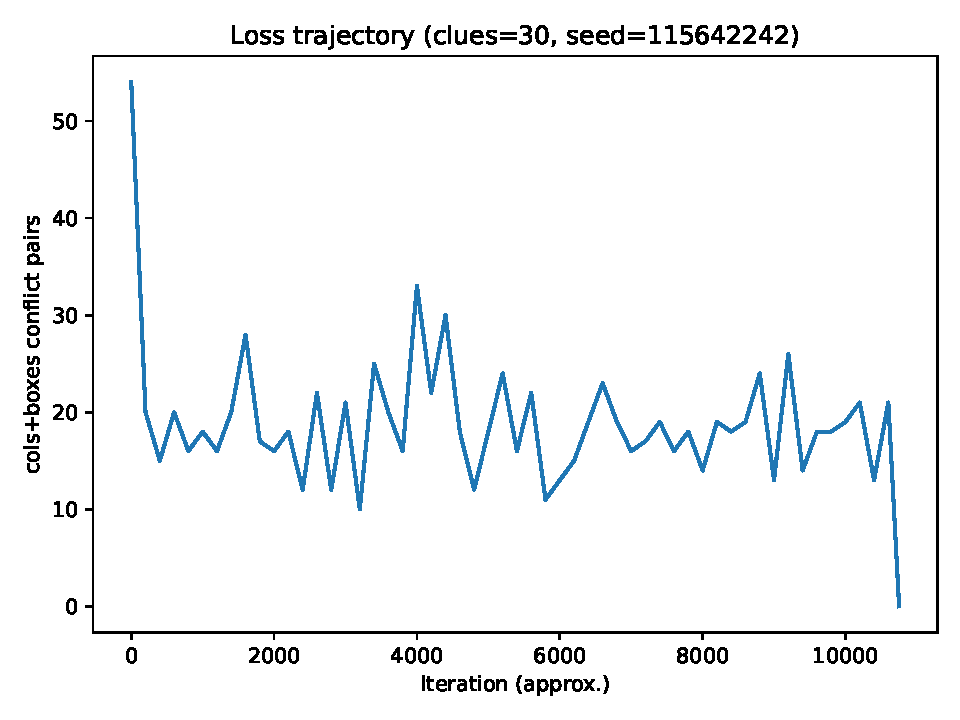
\includegraphics[width=0.75\linewidth]{loss_curve.pdf}
\caption{Conflict trajectory for the stepwise row-swap heuristic on the fast-carved $30$-clue instance with puzzle seed $955101029$ (solve seed $2638744256$), from the row-wise random initialisation on restart $0$.}
\label{fig:loss}
\end{figure}

\section{Powers-of-two experiments}
\label{app:powers-two}
An alternative maps digits \(d\in\{1,\dots,9\}\) to powers of two,
\[
d \longmapsto 2^{d-1} \in A := \{1,2,4,\dots,256\}.
\]
If every cell variable is restricted to \(A\), then the condition that a row, column, or box contains each digit exactly once is equivalent to a single sum constraint
\[
\sum_{(r,c)\in g} \beta_{r,c} = 1+2+\cdots+256 = 2^9-1 = 511,
\]
for each unit \(g\). This replaces the pairwise penalties by \(27\) residuals of the form
\[
r_g(\beta) := 511 - \sum_{(r,c)\in g}\beta_{r,c}.
\]
For a prime \(p\), one can then study the objective
\[
L_p(\beta) := \sum_g |r_g(\beta)|_p,
\]
optionally together with a regulariser that encourages \(\beta_{r,c}\in A\) and enforces the clues.

Archived local-search experiments with this encoding were run on \(50\) Euler Project Problem \(96\) puzzles. Table~\ref{tab:powers-two-results} summarises the outcomes. None of these runs found a valid completion.

\begin{table}[t]
\centering
\small
\begin{tabular}{@{}p{0.14\linewidth}p{0.44\linewidth}p{0.10\linewidth}p{0.24\linewidth}@{}}
\toprule
Experiment & Setting & Solved & Summary \\
\midrule
E1 & Greedy cell-swap on \(15\) primes, \(50\) puzzles, \(3\) random initialisations per puzzle--prime pair (\(2250\) runs) & \(0/2250\) & Mean lift \(0.003\); mean \(12.5\) steps \\
E2 greedy & Greedy cell-swap on the \(5\) strongest E1 primes, again with \(50\) puzzles and \(3\) initialisations (\(750\) runs) & \(0/750\) & Mean lift \(0.009\); mean \(19.3\) steps \\
E2 SA & Simulated annealing on the same \(750\) runs & \(0/750\) & Mean lift \(0.000\); mean \(5000\) steps \\
\bottomrule
\end{tabular}
\caption{Archived local-search results for the powers-of-two encoding. The E1 prime sweep used primes \(2,3,5,7,11,13,17,23,47,73,97,127,257,521,2311\).}
\label{tab:powers-two-results}
\end{table}

\clearpage
\section*{Funding}
This research was supported by an Australian Government Research Training Program Scholarship.

\section*{Compliance with ethical standards}
This article does not contain any studies with human participants or animals performed by the author.

\section*{Conflict of interest}
The author declares that he has no conflict of interest.

\section*{Author contributions}
This is a single-author paper. The author is responsible for the conceptual development, proofs, implementation, and writing.

\section*{Code and data availability}
The Python implementation used for the heuristic experiments is publicly available at:
\begin{quote}\small
\url{https://github.com/solresol/sudoku-padic-regression}\\
Dataset archive: \href{https://huggingface.co/datasets/gregb/sudoku-padic-regression-experiments}{Hugging Face dataset}\\
Revision: \texttt{ba49a8b2e51670f66db624d814d3f31678881b93}\\
Scripts: \path{code/padic_sudoku_regression.py}, \path{code/run_experiments.py}
\end{quote}
The submitted source package includes the experiment CSV files, puzzle seeds, trace puzzle and solution files, and figure source used for Table~\ref{tab:results} and Figure~\ref{fig:loss}.

\subsection*{Interactive demonstration}
A browser-based demonstration of the construction is available at
\begin{quote}\small
\url{https://padic-logic.symmachus.org}
\end{quote}
It has two modes, and all computation runs client-side. The all-different mode compiles a Sudoku or list-colouring instance into the signed \(p\)-adic residual objective of Definition~\ref{def:list-loss} on the native cell variables, evaluates the genuine \(p\)-adic norms (with \(p=11\)), and animates the row-swap and Zubarev-walk heuristics of Appendix~\ref{app:heuristics} until the column/box conflict count reaches its floor; on an unsatisfiable instance the search visibly settles at a minimum-conflict state. The Boolean mode illustrates the clause-reward remark of Section~\ref{construction}: it compiles a CSP to ternary clauses, displays each clause as a forbidden affine equality \(u_C^\top x\neq t_C\), and searches for satisfying assignments in the browser.

\begin{thebibliography}{99}

\bibitem{baker2025padic}
G. Baker, S. McCallum, and D. Pattinson.
\newblock Linear regression in \(p\)-adic metric spaces.
\newblock \emph{p-Adic Numbers, Ultrametric Analysis and Applications} 17(4), 333--347 (2025).
\newblock \url{https://doi.org/10.1134/S2070046625040016}

\bibitem{baker2026nphard}
G. Baker.
\newblock Expressivity and NP-hardness of \(p\)-adic linear regression.
\newblock \emph{p-Adic Numbers, Ultrametric Analysis and Applications} 18(2), 210--216 (2026).
\newblock \url{https://doi.org/10.1134/S2070046626020081}

\bibitem{knuth2000dancing}
Donald E. Knuth.
\newblock \emph{Dancing Links}.
\newblock \emph{Millennial Perspectives in Computer Science}, 187--214, 2000.
\newblock Also available as arXiv:cs/0011047.
\newblock \url{https://doi.org/10.48550/arXiv.cs/0011047}

\bibitem{simonis2005sudoku}
Helmut Simonis.
\newblock \emph{Sudoku as a Constraint Problem}.
\newblock In \emph{Modelling and Reformulating Constraint Satisfaction Problems}, Fourth International Workshop, Sitges (Barcelona), Spain, October 1, 2005.
\newblock \url{https://citeseerx.ist.psu.edu/document?doi=4f069d85116ab6b4c4e6dd5f4776ad7a6170faaf}

\bibitem{lynce2006sudoku}
In\^es Lynce and Jo\"el Ouaknine.
\newblock \emph{Sudoku as a {SAT} Problem}.
\newblock In \emph{Proceedings of the Ninth International Symposium on Artificial Intelligence and Mathematics (ISAIM 2006)}, 2006.
\newblock \url{https://people.mpi-sws.org/~joel/publications/sudoku05abs.html}

\bibitem{yato-seta}
T.~Yato and T.~Seta.
\newblock Complexity and completeness of finding another solution and its application to puzzles.
\newblock \emph{IEICE Transactions on Fundamentals}, 86-A(5):1052--1060, 2003.

\bibitem{zubarev2025padic}
A. P. Zubarev.
\newblock \(p\)-Adic polynomial regression as alternative to neural network for approximating \(p\)-adic functions of many variables.
\newblock \emph{p-Adic Numbers, Ultrametric Analysis and Applications} 17(4), 413--420 (2025).
\newblock \url{https://doi.org/10.1134/S2070046625040065}

\bibitem{mihara2026polyreg}
T. Mihara.
\newblock \(p\)-adic polynomial regression detecting digitwise noise.
\newblock \emph{p-Adic Numbers, Ultrametric Analysis and Applications} 18(1), 33--47 (2026).
\newblock \url{https://doi.org/10.1134/S2070046626010036}

\bibitem{mihara2026digitwise}
T. Mihara.
\newblock \(p\)-adic linear regression for random sampling with digitwise noise.
\newblock arXiv:2604.13137 (2026).
\newblock \url{https://arxiv.org/abs/2604.13137}

\bibitem{mihara2026manifoldgames}
T. Mihara.
\newblock \(p\)-adic manifold learning and benchmark tasks from impartial games.
\newblock arXiv:2605.04374 (2026).
\newblock \url{https://arxiv.org/abs/2605.04374}

\bibitem{mihara2026forcing}
T. Mihara.
\newblock Generalisation of Baker's forcing method to arbitrary prime and NP-hardness of several \(p\)-adic optimisations.
\newblock arXiv:2607.06092 (2026).
\newblock \url{https://arxiv.org/abs/2607.06092}

\bibitem{hua1983negative}
T. A. Hua and R. F. Gunst.
\newblock Generalized ridge regression: a note on negative ridge parameters.
\newblock \emph{Communications in Statistics - Theory and Methods} 12(1), 37--45 (1983).
\newblock \url{https://doi.org/10.1080/03610928308828440}

\bibitem{kobak2020negative}
D. Kobak, J. Lomond, and B. Sanchez.
\newblock The optimal ridge penalty for real-world high-dimensional data can be zero or negative due to the implicit ridge regularization.
\newblock \emph{Journal of Machine Learning Research} 21(169), 1--16 (2020).
\newblock \url{https://www.jmlr.org/papers/v21/19-844.html}

\bibitem{patil2024oodridge}
P. Patil, J.-H. Du, and R. Tibshirani.
\newblock Optimal ridge regularization for out-of-distribution prediction.
\newblock In \emph{Proceedings of the 41st International Conference on Machine Learning}, \emph{Proceedings of Machine Learning Research} 235, 39908--39954 (2024).
\newblock \url{https://proceedings.mlr.press/v235/patil24a.html}

\bibitem{wiesel2008gaussian}
A. Wiesel, Y. C. Eldar, and A. Yeredor.
\newblock Linear regression with Gaussian model uncertainty: Algorithms and bounds.
\newblock \emph{IEEE Transactions on Signal Processing} 56(6), 2194--2205 (2008).
\newblock \url{https://doi.org/10.1109/TSP.2007.914323}

\bibitem{cannon2009negative}
A. J. Cannon.
\newblock Negative ridge regression parameters for improving the covariance structure of multivariate linear downscaling models.
\newblock \emph{International Journal of Climatology} 29(5), 761--769 (2009).
\newblock \url{https://doi.org/10.1002/joc.1737}

\end{thebibliography}

\end{document}
